The Leap Motion Controller, created by Leap Motion Inc, is a vision-based gesture recognition system, first released in 2013 with several new versions released in the following
years. As mention in section~\vref{sec:design_leapmotion} the Leap Motion Controller is an attractive choice because of it accessibility and affordability and was thus 
selected as the gesture recognition system of choice for the design review application. 
This chapter is based on the Leap Motion Controller documentation (see \citet{LeapMotion2016}) for the Orion software (i.e version 3.2 of the Leap motion software), 
and aims to highlight the important conceptual foundation for using the Leap Motion Controller in this thesis' design review application.

% The controller, approximately the size of a box of matches, allows for the precise and fluid tracking of multiple hands, fingers, and small objects in free space with 
% sub-millimeter accuracy~\citep{Guna2014}.
\begin{figure}%[h!] %[H]
	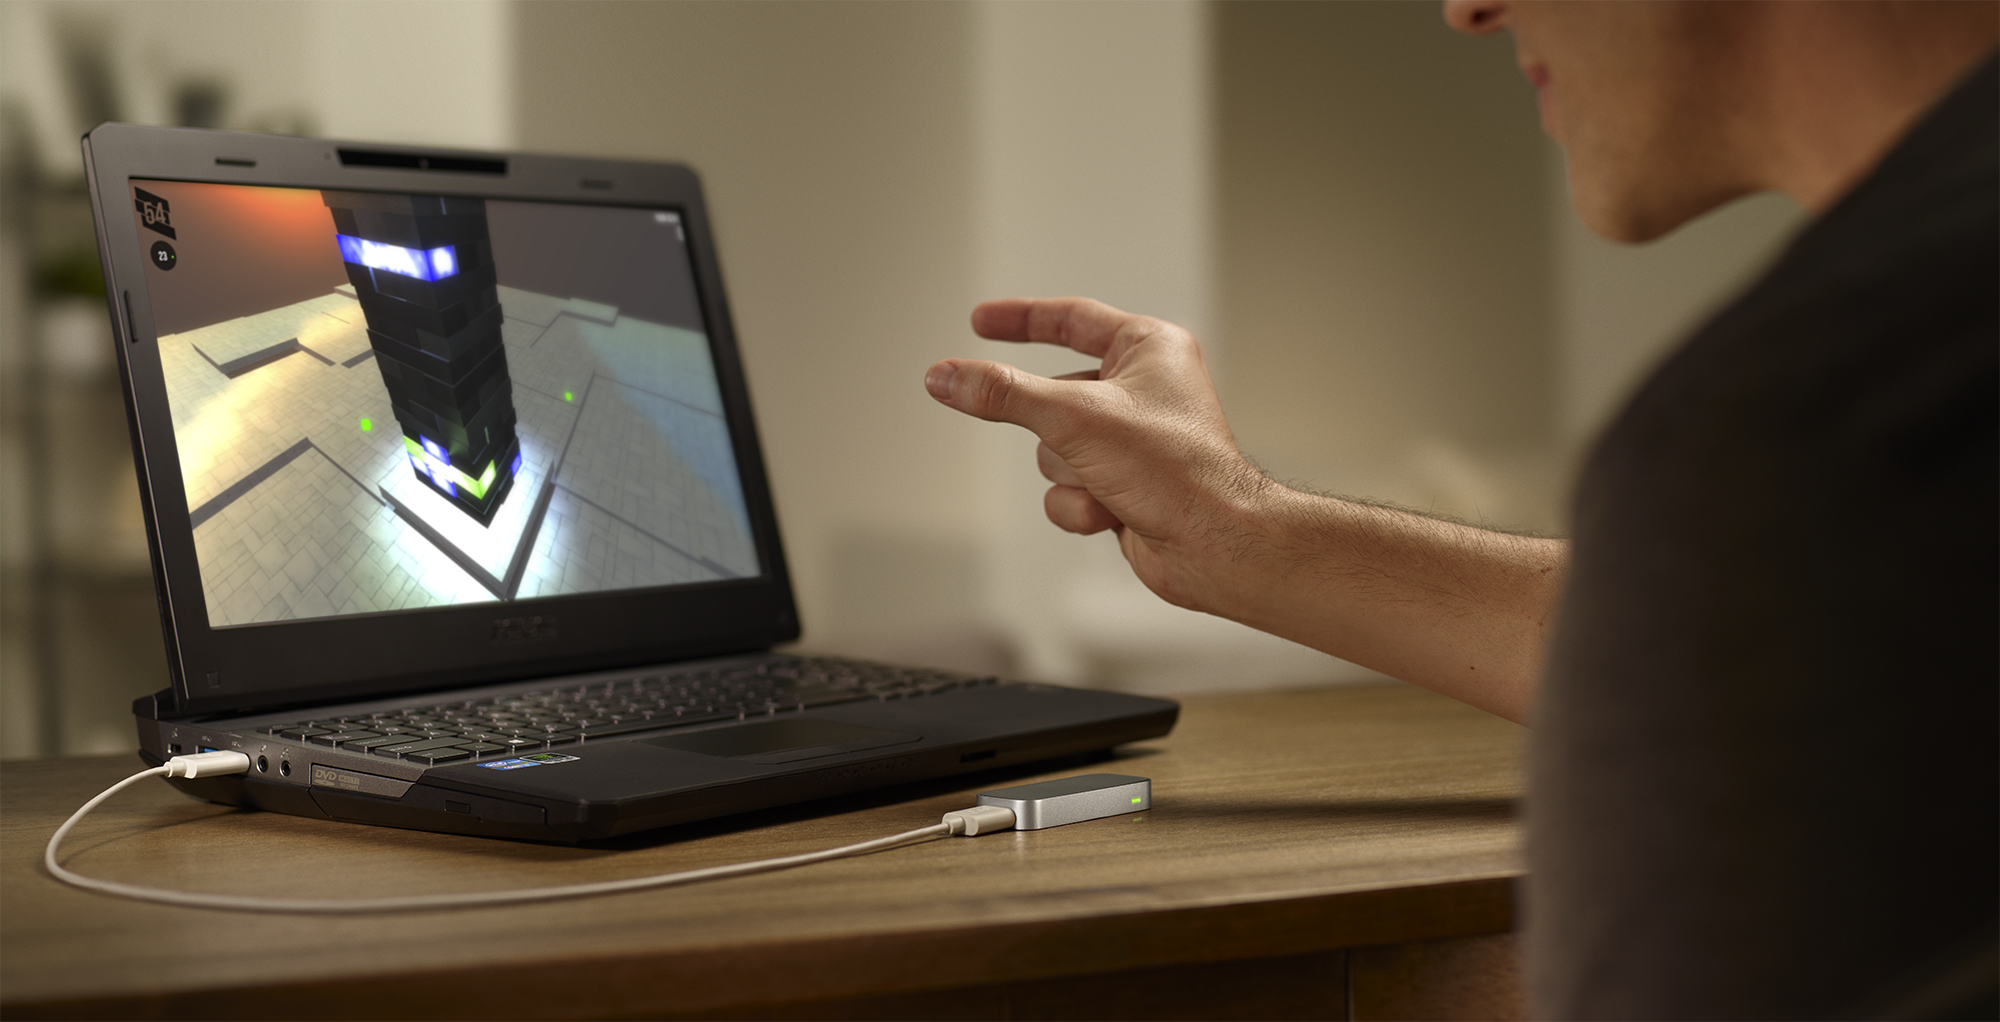
\includegraphics[width=\linewidth]{pictures/leapmotion2.png}
	\caption[The Leap Motion Controller]{The Leap Motion Controller is a vision-based gesture recognition devices that can be placed on a table top to observe the users hands.}
	\label{fig:leapmotion}
\end{figure} 

\section{Physical properties}
The Leap Motion Controller (see fig.~\vref{fig:leapmotion} and~\vref{fig:leapmotion2}) contains two stereoscopic cameras, with a field of view of about 150 degrees, 
in addition to three infrared LEDs. 
These lights periodically emit infrared light pulses at a wavelength of 850 nanometers, thus outside the visible light spectrum, which light up about the 
area in front of the controller. During these pulses grayscale stereo images are also captured, with an effective range from approximately 25 to 600 millimeters above the device.
After this the images are sent to the tracking software, where the images are analyzed to construct 3D representations of the captured 2D images (by comparing offsets), and
compensate for static background objects and ambient environmental lighting. 
The data derived from the pictures are also combined with an internal model of the human hand to help cope with challenging tracking conditions.

\begin{figure}%[h!] %[H]
	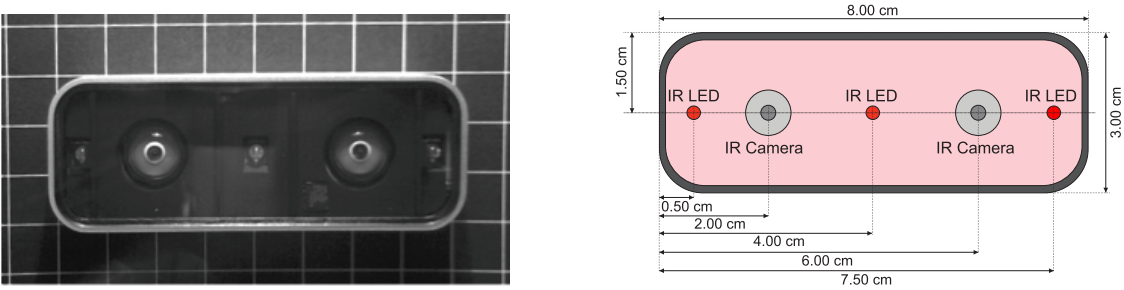
\includegraphics[width=\linewidth]{pictures/LMC_measures.png}
	\caption[Visualization of a Leap Motion Controller]{Visualization of a Leap Motion Controller, with Infrared Imaging (left) and a Schematic View (right)~\citep{Weichert2013}.}
	\label{fig:leapmotion2}
\end{figure} 

\section{The Leap API}
The controller itself can be accessed and programmed through high level Application Programming Interfaces (APIs), with support for a variety of programming languages, 
including C++, C\#, Objective-C, Java, JavaScript and Python. Although the API is programmed almost exclusively in C, access through a variety of other languages 
is achieved by virtue of various "wrapper libraries", which exposes and translates functions from their respective languages into the corresponding C function.
In addition to this, the Leap Motion SDK also features integration with commercial game engines such as Unity and the Unreal Engine. 
This section will cover important concepts in the Leap API, which are thoroughly used in the thesis implementation.

\subsection{Integration with the Unity editor}
To use Leap Motion in a Unity project one can simply import the Leap Motion Core Asset Package, which includes the necessary scripts and components to utilize Leap Motion in the 
project. In addition to this Leap Motion also offers different modules, which contain several useful assets. 
Several of the assets provided by Leap Motion can often be included directly in the scene, such as LeapHandController from the core module and the hand model prefabs 
from the hands module.
The LeapHandController is arguably the most important prefab in the Leap Motion Asset Packages and is responsible for representing the Leap Motion device 
in the scene, which is important with regard to where the hand models, when active, are positioned relative to the camera. 
LeapHandController is also important as it has the LeapServiceProvider script, which contain several key function, as a component.

The hand model prefabs are also useful assets, as - when used correctly- they can be present in the scene and mimic what the user's hands are doing.
This helps the user get visual feedback on what the controller is capturing and should also make it easier for the user to 
hold his or her hands in an optimal position for the Leap Motion Controller to capture.


\subsection{The Hand Abstractions}
% The Leap Motion API offers many convenient abstractions for relevant properties when detecting and tracking hands.
% Hands are the main entity tracked by the Leap Motion controller, and it maintains an inner model of the human hand and validates the data from 
% its sensors against this model. This allows the controller to track finger positions even when some fingers are not visible from the Leap Motion Controllers point of view.

The Hand class represents a physical hand detected by the Leap Motion Controller, and is perhaps one of the most central abstractions in the Leap Motion API. 
A Hand object provides access to lists of its pointables as well as attributes describing the hand position, orientation, and movement.
Each hand-object also have object-representations for its fingers, palm etc, each with its own data.
One common way to access the hands are through the \textit{frame object}, which is an object-oriented representation of the last captured frame of the device.
Each of these frame objects contain a list called \texttt{hands}, which contains a hand-object per detected and tracked hand in that frame.
These hand objects have their own instance variables, which provide useful information about the properties of the hand (e.g~its position and velocity relative to the Leap Motion
Controller). Some examples of what variables the hand objects contain can be seen in table~\vref{tab:hand_variables}

% \begin{itemize}
% \item isRight, isLeft — Whether the hand is a left or a right hand.
% \item Palm Position — The center of the palm measured in millimeters from the Leap Motion origin.
% \item Palm Velocity — The speed and movement direction of the palm in millimeters per second.
% \item Palm Normal — A vector perpendicular to the plane formed by the palm of the hand. The vector points downward out of the palm.
% \item Direction — A vector pointing from the center of the palm toward the fingers.
% \item grabStrength, pinchStrength — Describe the posture of the hand.
% \item Motion factors — Provide relative scale, rotation, and translation factors for movement between two frames.
% \end{itemize}

\begin{table}[]
\centering
\label{tab:hand_variables}
\begin{tabular}{p{2.5cm}| p{8cm}}
	\textbf{Variable name} &  \textbf{Description} \\ \hline
	isRight, isLeft & Whether the hand is a left or a right hand. \\ \hline
	palmPosition    & The center of the palm measured in millimeters from the Leap Motion origin. \\ \hline
	palmVelocity    & The speed and movement direction of the palm in millimeters per second.  \\ \hline
	palmNormal      & A vector perpendicular to the plane formed by the palm of the hand. The vector points downward out of the palm.  \\ \hline
	direction       & A vector pointing from the center of the palm toward the fingers.  \\ \hline
	grabStrength    & Describe the posture of the hand.  \\ \hline
	pinchStrength   & Describe the posture of the hand.  \\ \hline
	motionFactors   & Provide relative scale, rotation, and translation factors for movement between two frames. 
\end{tabular}
\caption{Some of the instance variables of the Leap API Hand class.}
\end{table}

Figure~\vref{table:annotation_visibility_code} shows an example derived from the MovementController.cs class in the design review implementation. 
This example highlights how hand objects can be acquired from the frame object, how we can e.g.~make sure its a left-hand
before proceeding, and how we can calculate a new position based on the hand position offset from the gesture origin.
Note that this code is incomplete and only meant as a somewhat compact example.

\begin{table}
\label{table:annotation_visibility_code}
\lstset{style=csharp}
\begin{lstlisting}

//Update() runs every frame (typically between 30 - 120 times per second)
void Update()
{
    Frame frame = LeapBehavior.getLastFrame();
    iBox = frame.InteractionBox; //Used for normalization
    for (int i = 0; i < frame.Hands.Count; i++)
    {
        Hand hand = frame.Hands[i]; 

        if (hand.IsLeft && leftHand.getGestureType() != HandState.NONE)
        {
            //Measure hand position from palm position
            Vector leapPoint = hand.StabilizedPalmPosition;
            
            //Converting from right hand to left hand coordinate convention
            leapPoint.z *= -1.0f; 

            //Normalizing the point
            Vector normPoint = iBox.NormalizePoint(leapPoint, false);
            
            if (gestureHand.getGestureType() == HandState.PALM_DOWN) 
            {
                //PALM_DOWN is the gesture to navigate up and down the y-axis          
                //The y-axis hand offset from origin:
                float y_offset = normPoint.y - gestureHand.GetGestureOriginPosition().y;

                //Calculate new player model position
                transform.position += transform.up * speed * y_offset * Time.deltaTime;
            }             
        }
    }
}
\end{lstlisting}
\caption[Accessing the Leap Motion Frame objects]{Accessing the Leap Motion Frame objects}
\end{table}

\subsection{The Coordinate System}
The Leap Motion API enables acquisition of the recognized object's position through Cartesian and spherical coordinate systems, 
which are used to describe positions in the controller's sensory space. The hand positions above the Leap Motion device are given as three dimensional
vectors on the form \{x, y, z\}, with origin being in the center of the Leap Motion surface (see~\vref{fig:leapmotion3}).  
Positional information, like the position of a hand, or the position of the tip of a finger, can be access in various ways. One way is to access the hands through the
Frame-object, and then find the relevant hand, palm, finger or finger-joint.

The Leap Motion API uses a right-handed coordinate convention, meaning that when the user is positioned in front of the Leap Motion Controller the x-axis grows more positive 
towards the right, the y-axis grows more positive upwards and the z-axis grows more positive towards the user (see~\vref{fig:leapmotion3}). 
As some frameworks, like the Unity engine, use a left-handed convention for their coordinate system, i.e that the z-axis grows more positive away from the 
user instead of towards, the Leap Motion API also does an appropriate convention to adhere to its software environment. 
The Leap Motion API also adhere to differences in units, as e.g Unity uses a default unit of meters, while the Leap Motion uses millimeters as default.

\begin{figure}%[h!] %[H]
	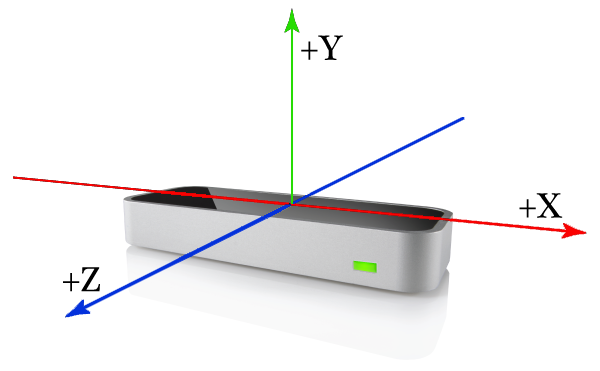
\includegraphics[width=\linewidth]{pictures/Leap_Axes.png}
	\caption[Leap Motion Coordinates]{The Leap Motion Coordinate System has its origin between the two cameras.}
	\label{fig:leapmotion3}
\end{figure} 

\subsection{The Detection Utilities}
To provide a common and high level interface to recognize gestures the Leap Motion API offers several detection utilities called \textit{detectors}.
Detectors are scripts in the core asset package that serve as basic building blocks for hand action detections, and can e.g.~detect whether a certain finger is extended or not
or which way the palm is facing. New detectors can also be created by extending
the \texttt{Detector} base class and implement logic that calls \texttt{Active()} when the detector turns on - i.e when a certain condition is met (e.g~a gesture is performed) - 
and \texttt{Deactivate()} when it turns off (i.e~ when the condition is no longer met).

Several of these detector can be chained together using a \textit{Logic Gate} to create more complex expressions. 
The \texttt{DetectorLogicGate} is itself a detector that logically combines two or more other detectors, using operations like AND, OR, NAND (not AND) and NOR (not OR), 
to determine its own state.
If one thus were to make a thumb's up-gesture, one could use a logic gate with an AND-configuration together with a detector for detecting whether or not the
thumb is extended and a detector for determining whether or not the thump if facing upward. 

The detectors also have some public variables that can be adjusted to find the optimal "gesture sensitivity". These include \textit{Period}, which determines how often 
the detector checks the hand state,
\textit{HandModel}, which refers to which hand model is being observed by the detector and several on-or-off values, 
which sets the thresholds for when the detector should be active (i.e the detector recognizes the property it's looking for) or off. 
These on and off values can especially be the subject of repeated adjustment, as it is deemed crucial to find a good
compromise between the two values (more on this in the implementation chapter). The detectors also has some public functions, with two of the most important ones being
\texttt{OnActivate()} and \texttt{OnDeactivate()}. \texttt{OnActivate()} is called by its detector when the detector turns on (activates), 
while \texttt{OnDeactivate()} is called when it turns off (deactivates). 

This outlines the primary means of creating gestures and connecting them to actions using the Leap Motion API. One can create gesture expressions, like the thumb's up-gesture
described above, using a Logic Gate with AND. This Logic Gate will only be active (on), while all of the detectors it references ("is hooked up to") are active, so in our example
only when the thumb is extended AND facing upwards. By then assigning a custom created function, e.g.~a function called "Accept", to the Logic Gate's OnActive-function we
ensure that this function is called only when the thumb's up-gesture is done correctly. 



% Technically, very few details are publicly known about the precise nature of the algorithms used due to patent and trade secret restrictions.

% \section{Important Leap components}




% Hands, fingers, palm, directions, frames, interaction box etc. 
% See \\
% https://developer.leapmotion.com/documentation/csharp/devguide/Leap\_Overview.html\#motion-tracking-data \\
% https://developer.leapmotion.com/documentation/csharp/devguide/Leap\_Coordinate\_Mapping.html\#map3d \\
% https://developer.leapmotion.com/documentation/csharp/devguide/Leap\_Hand.html \\


% \section{Detectors - The building blocks of gesture recognition}
% The detector scripts. How they can be combined. Logic gates. 
% See https://developer.leapmotion.com/documentation/unity/unity/Unity\_DetectionUtilities.html

% \section{Integration with the Unity editor}
% How the pieced fit together. How the stuff is organized (e.g the modules).
% See https://developer.leapmotion.com/documentation/unity/index.html